\documentclass[a4]{article}
\usepackage[czech]{babel}
\usepackage[utf8]{inputenc}
\usepackage{listings}
\usepackage{hyperref}
\usepackage{color}
\usepackage{amsmath}
\usepackage{multicol}
\usepackage{titlesec}
\usepackage{graphicx}
\graphicspath{ {images/} }

\usepackage{relsize}

\setlength{\parskip}{1em}

\definecolor{dkgreen}{rgb}{0,0.6,0}
\definecolor{gray}{rgb}{0.5,0.5,0.5}
\definecolor{mauve}{rgb}{0.58,0,0.82}

\lstset{frame=tb,
  language=Octave,
  aboveskip=3mm,
  belowskip=3mm,
  showstringspaces=false,
  columns=flexible,
  basicstyle={\small\ttfamily},
  numbers=none,
  numberstyle=\tiny\color{gray},
  keywordstyle=\color{blue},
  commentstyle=\color{dkgreen},
  stringstyle=\color{mauve},
  breaklines=true,
  breakatwhitespace=true,
  tabsize=3
}

\newcommand{\HRule}{\rule{\linewidth}{0.5mm}}

\titleformat{\section}
{\normalfont\LARGE\bfseries}{\thesection}{1em}{}
\titleformat{\subsection}
{\normalfont\Large\bfseries}{\thesubsection}{1em}{}
\titleformat{\subsubsection}
{\normalfont\large\bfseries}{\thesubsubsection}{1em}{}
\titleformat{\paragraph}[runin]
{\normalfont\large\bfseries}{\theparagraph}{1em}{}
\titleformat{\subparagraph}[runin]
{\normalfont\large\bfseries}{\thesubparagraph}{1em}{}

\title
{
\begin{figure}[h]

\includegraphics[scale=0.5]{zcuLogo}
\centering
\end{figure}
\textsc{\Huge{Semestrální práce}}\\*\LARGE{KIV-SU}\\\textbf{\huge{Strojové učení}}
}

\author{Jakub Zíka - A15N0087P\\zikaj@students.kiv.zcu.cz}
\date{\today}

\begin{document}
\maketitle
\newpage

\tableofcontents{}
\newpage

\section{Zadání}
Navrhněte téma zadání semestrální práce související s oblastí strojového učení. Cílem práce je prohloubit znalosti studenta v oblasti kognititvních systémů pomocí nabytých zkušeností ze semetrální práce.

\subsection{Vybrané zadání}
Sestrojte klasifikátor \textit{Support Vector Machines}, dále už jen \textit{SVM}, který bude skrze osobní údaje pasažérů lodi Titanic klasifikovat, zda daná osoba přežije či nepřežije potopení lodi. Data obsahují následující příznaky:

\begin{enumerate}
	\item survived : přežil/nepřežil (1/0)
	\item pclass : socio-ekonomická třída pasažéra (1=vyšší, 2=střední, 3=nižší)
	\item name : jméno
	\item sex : pohlaví
	\item age : věk
	\item sibsp : počet sourozenců, partnerů na palubě (příbuzní stejné generace)
	\item parch : počet rodičů, dětí na palubě (příbuzní odlišné generace)
	\item ticket : ID lístku
	\item fare : cena lístku
	\item cabin : číslo kajuty
	\item embarked : přístav nalodění (C=Cherbourg, Q=Queenstown, S=Southampton)
\end{enumerate}

\begin{figure}[!ht]
	\centering
		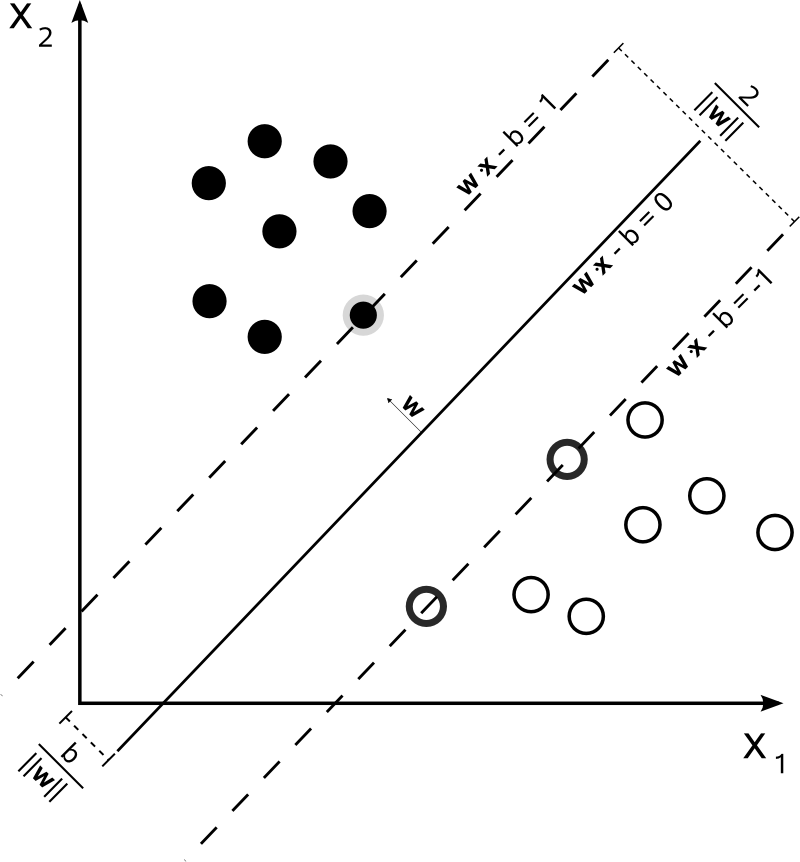
\includegraphics[scale=0.25]{images/svm_vectors}
	\caption{Maximální pás bez bodů trénovací množiny \cite{svm_wiki}}
	\label{fig:svm_vectors}
\end{figure}

\section{Teoretický úvod}

\subsection{Support Vector Machines}
Algoritmy strojového se skládají z \textit{trénovací množiny} a \textit{rozhodovací hranice}. Rozhodovací hranici můžeme též nazývat \textit{hypotéza}. Algoritmy tedy dělíme na \textit{učení s učitelem} (máme odpovědi) a \textit{učení bez učitele} (nemáme odpovědi).
\\\\
Každý vzorek $\vec{x}$ trénovací množiny je tvořen množinou příznaků $$\vec{x} = [x_1,x_2,...x_n],$$kde \textit{n} je počet příznaků. Hypotéza má tvar $h:x \rightarrow y$ což znamená, že hypotéza je zobrazení \textit{x} do \textit{y}. Hypotézu tvoří modelovací parametry $$\vec{\Theta},$$které nám umožňují nastavit rozhodovací hranici. Jejich hodnoty předem neznáme a získáme je trénováním.\cite{andrew},\cite{svm_zcu}

\subsubsection{Lineární rozhodovací hranice}
SVM je metoda strojového učení, která hledá v trénovací množině umístění optimální nadroviny. Tato nadrovina slouží k rozdělení bodů projekce na dvě třídy. V tomto rozdělení je požadováno aby minimum vzdáleností bodů od této nadroviny bylo co největší. Chceme tedy, aby nadrovina měla po obou stranách co nejširší pás bez bodů. K popisu těchto pásů slouží pomocné vektory (\textit{Support Vectors}) (viz Obr.:\ref{fig:svm_vectors}).
\cite{svm_zcu}

\subsubsection{Cenová funkce}
Metoda SVM je vylepšenou verzí \textit{logistické regrese}. Ovšem, na rozdíl od cenové funkce logistické regrese nám SVM nevrací pravděpodobnost, ale rovnou příslušnost klasifikovaného vzorku k třídě 1 nebo 0. Zde vidíme \textit{cenovou funkci} logistické regrese:
$$
\min_{\vec{\Theta}} \frac{1}{m}[\sum_{i=1}^{m}y^{(i)}(-\log h_{\vec{\Theta}}(x^{(i)}))+(1-y^{(i)})(-\log(1-h_{\vec{\Theta}}(x^{(i)})))]+\frac{\lambda}{2m}\sum_{j=1}^{n}\Theta_{j}^{2}.
$$
\noindent Cenová funkce SVM pak vypadá následovně:
$$
\min_{\vec{\Theta}} C \sum_{i=1}^{m}[y^{(i)} Cost_1 (\vec{\Theta}^T x^{(i)})+(1-y^{(i)}) Cost_0 (\vec{\Theta}^T x^{(i)})] + \frac{1}{2} \sum_{j=1}^{n}\Theta_{j}^{2},
$$
\noindent kde $Cost_1$ funkce pro y = 1 je
$$
\log(\frac{1}{1 + e^{-\Theta^{T}x}})
$$
\noindent a funkce $Cost_0$ funkce pro y = 0 je
$$
\log(1-\frac{1}{1 + e^{-\Theta^{T}x}}).
$$
\noindent Optimalizací cenové funkce získáme hodnoty parametrů $\vec{\Theta}$, které určují tvar hypotézy.
\\\\
Hodnota $C$ je regularizační faktor, který ovlivňuje výběr hypotézy. Rozumně vybraná hodnota pak umožní dělat ve výběru hypotézy kompromisy v extrémních případech rodělení tříd v trénovací množině:

\begin{enumerate}
	\item $C$ - vysoké = malá odchylka, velký rozptyl (malá $\lambda$), hrozí \textit{overfitting}
	\item $C$ - malé = velká odchylka, malý rozptyl (velká $\lambda$), hrozí \textit{undefitting}
\end{enumerate}

\begin{figure}[!ht]
	\centering
		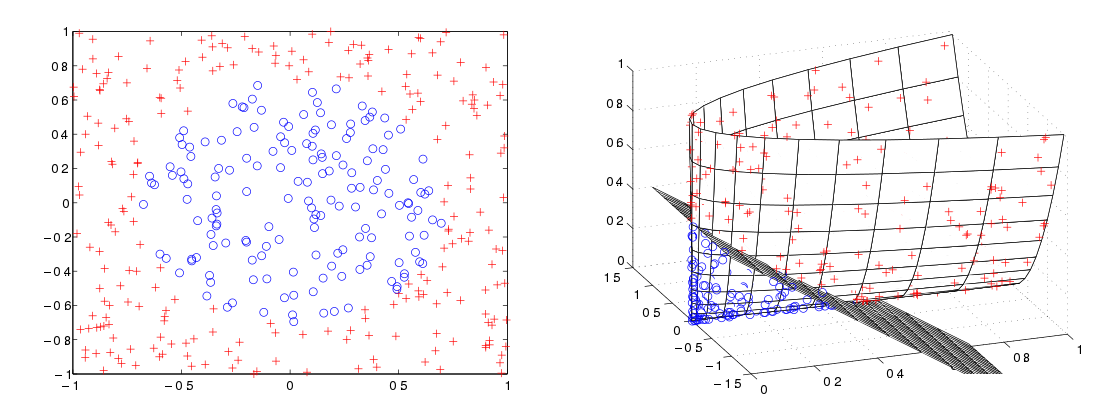
\includegraphics[width=\textwidth]{images/linear_nonlinear}
	\caption{Ukázka lineárně neseparabilních a separabilních dat.\cite{svm_wiki}}
	\label{fig:linear_nonlinear}
\end{figure}

\subsubsection{Nelineární rozhodovací hranice}
Máme-li trénovací množinu, pro kterou je rozhodovací hranice nelineární (viz. Obr.:\ref{fig:linear_nonlinear}), musíme použít metodu jader (\textit{Kernels}). Zavedeme si \textit{i} pomocných bodů tzv. \textit{landmarky}. Každý landmark $\vec{l^{(i)}}$ nese hodnotu vzdálenosti od ostatních prvků trénovací množiny. Ke každému prvku $\vec{x^{(m)}}$ trénovací množiny spočteme podobnost $f_{i}$ s každým landmarkem $\vec{l^{(i)}}$. Pro každý prvek trénovací množiny tak dostaneme vektor podobnosti $\vec{f^{(m)}}$. Podobnost počítáme následovně:
$$
f_{i}(\vec{x^{(m)}},\vec{l^{(i)}}) = exp(-\frac{||\vec{x^{(m)}} - \vec{l^{(i)}}||}{2\sigma^2})
$$

\noindent a vektor podobnosti pak bude vypadat:

$$\vec{f^{(m)}} = [f_{1},f_{2},f_{3},...,f_{i}].$$

\noindent Jádrem se nazývá funkce počítání podobnosti. V tomto případě je jádro \textit{Gaussové}. Parametr \textit{sigma} nám určuje míru podobnosti. Máme i jiné funkce jádra jako například \textit{Polynomiální} nebo \textit{Lineární}. Lineární jádro je předchozí případ lineárně separabilních dat.\cite{svm_robots},\cite{svm_wiki}

\begin{figure}[!ht]
	\centering
		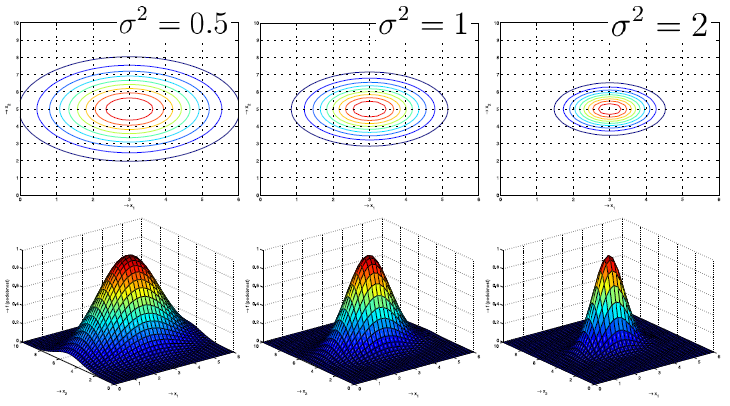
\includegraphics[width=\textwidth]{images/sigma}
	\caption{Míra podobnosti v závislosti na parametru $\sigma$.\cite{svm_zcu}}
	\label{fig:sigma}
\end{figure}

\noindent Podobnost se určuje na grafu podobnosti (viz Obr.:\ref{fig:sigma}) tak, že čím je zkoumaný prvek blíže globálnímu maximu gaussovského klobouku, tím míra podobnosti narůstá. Jak moc je graf špičatý, či plochý závisí právě na parametru $\sigma$. Vlastnosti velikosti paramteru $\sigma$:

\begin{itemize}
	\item $\sigma$ - velká = menší odchylka, vetší rozptyl (příznaky $f_i$ se mění prudčeji)
	\item $\sigma$ - malá = větší odchylka, menší rozptyl (příznaky $f_i$ se mění pomaleji)
\end{itemize}

\subsubsection{Cenová funkce s jádry}
Při použití gaussového jádra máme předpočítaný vektor podobnosti pro každý prvek trénovací množiny. To znamená, že vektor podobnosti může reprezentovat daný prvek trénovací množiny. Cenouvou funkci tedy můžeme pozměnit do tvaru:
$$
\min_{\vec{\Theta}} C \sum_{i=1}^{m}[y^{(i)} Cost_1 (\Theta^T \vec{f^{(i)}})+(1-y^{(i)}) Cost_0 (\Theta^T \vec{f^{(i)}})] + \frac{1}{2} \sum_{j=1}^{n}\Theta_{j}^{2}.
$$
\noindent Pozor, gaussové jádro je citlivé na velké rozdíly hodnot mezi jednotlivými příznaky. Je dobré příznakový vektor nejdříve naškálovat a až poté počítat cenovou funkci.

\subsection{Sequential minimal optimization}
SMO je algoritmus objevený Johnem Plattem v roce 1998. Tento algoritmus se osvědčil v SVM. Budeme jím počítat cenovou funkci. Za pomoci \textit{Lagrangoevých multiplikátorů} můžeme říct, že $\Theta(\alpha)=\sum_{i}\alpha_{i}y_{i}z_{i}$, kde $\alpha_i$ jsou Lagrangeovy multiplikátory a $z_{i}=\phi(x_{i})$.
\\\\
Platt toto vylepšení poté využije jako:
$$
F_i =w(\alpha) . z_i - y_i = \sum_{j}\alpha_{j}y_{j}k(x_i,x_j)-y_{i},
$$
kde $k(x_i,x_j)$ je jádro. Dostáváme tvar parciální derivace:
$$
L = \frac{1}{2}w(\alpha).w(\alpha)-\sum_{i}\alpha_{i}-\sum_{i}\alpha_{i}\delta_{i}+\sum_{i}\mu_{i}(\alpha_{i}-C)-\beta\sum_{i}\alpha_{i}y_{i},
$$
$$
\frac{\partial L}{\partial \alpha_{i}}=(F_{i}-\beta)y_{i}-\delta_{i}+\mu_{i}=0.
$$
Podle \textit{Karush-Kuhn-Tucker (KKT)} dostaneme podmínky, které musí daný výraz splňovat:
$$
(F_i-\beta)y_{i} \geq -\tau \Rightarrow \alpha_{i} = 0,
$$
$$
|(F_i-\beta)| \leq \tau \Rightarrow 0 < \alpha_{i} < C,
$$
$$
(F_i-\beta)y_{i} \leq \tau \Rightarrow \alpha_{i} = C.
$$
Platt poté definuje výstupní chybu i-tého prvku jako:
$$
E_{i} = F_{i} - \beta,
$$
kde $\beta$ je prahový paramter. V Plattově pseudokódu po určení chyby vybíráme dva indexy $i_1$ a $i_2$ pro výběr multiplikátorů $\alpha_{i_1}$ a $\alpha_{i_2}$. Metody, jak správně vybrat indexy, jsou popsány v originálním článku z roku 1998. Celý algoritmus tedy funguje ve dvou smyčkách. Vnější smyčka vybírá index $i_2$ a pro index $i_2$ vybírá vnitřní smyčka index $i_1$. Vnější smyčka jde přes všechny prvky trénovací množiny, které narušily podmínky optimality. Nejprve pouze přes ty, které nanerušili horní ani dolní hranici. V každém průběhu, je-li to vyžadováno, je chyba $E_i$ aktualizována.\cite{smo_platt},\cite{andrew}

\noindent Dále je nutné si spočítat horní a dolní hranici. Pokud se $y_{i_1}$ nerovná $y_{i_2}$ pak:
$$
L=max(0,\alpha_2 - \alpha_1) ; H=min(C, C+\alpha_2 - \alpha_1)
$$
jinak:
$$
L=max(0,\alpha_2 + \alpha_1 - C) ; H=min(C, \alpha_2 + \alpha_1).
$$
\noindent Druhá derivace cílové funkce podél diagonály může být vyjádřena jako:
$$
\eta=K(\vec{x_1},\vec{x_1}) + K(\vec{x_2},\vec{x_2}) -2K(\vec{x_1},\vec{x_2}).
$$
\noindent Za normálních okolností bude cílová funkce pozitivně definitní, bude existovat
minimum ve směru lineárního omezení rovnosti a $\eta$ bude větší než nula. V
tomto případě SMO vypočítá minimum ve směru omezení:
$$
\alpha_{2}^{new,cliped} = \alpha_{2}+\frac{y_{2}(E_{1}-E_{2})}{\eta}.
$$
\noindent Teď si vyjádříme $s=y_{1}y_{2}$. Potom se $\alpha_1$ počítá:
$$
\alpha_{1}^{new}=\alpha_{1}+s(\alpha_{2}-\alpha_{2}^{new,clipped}).
$$
\noindent Dále si musíme vytvořit vzorce pro výpočet prahu. Práh $\beta$ je počítán po každém provedeném vnitřním cyklu. Celkový práh je složen z $\beta_1$, který  je ovlivněn chybou $E_1$, a $\beta_2$, který je ovlivněn chybou $E_2$. Následující práh $\beta_1$ je platný, pokud nová $\alpha_{1}$ není v mezích, protože nutí výstup z SVM být $y_1$, když vstup je $x_1$:
$$
\beta_1=E_1+y_1(\alpha_1^{new}-\alpha_{1})K(\vec{x_1},\vec{x_1})+y_2(\alpha_2^{new}-\alpha_2)K(\vec{x_1},\vec{x_2})+\beta.
$$
\noindent Předchozí trvrzení pro $\beta_1$ platí i pro $\beta_2$. Následující práh $\beta_2$ je platný, pokud nová $\alpha_{2}$ není v mezích, protože nutí výstup z SVM být $y_2$, když vstup je $x_2$:
$$
\beta_2=E_2+y_1(\alpha_1^{new}-\alpha_{1})K(\vec{x_1},\vec{x_2})+y_2(\alpha_2^{new}-\alpha_2)K(\vec{x_2},\vec{x_2})+\beta.
$$
\noindent Pokud oba prahy $\beta_1$ i $\beta_2$ jsou platné, jsou si rovny. Když oba nové Lagrangeovy multiplikátory jsou v mezích a pokud L není rovno H, pak interval mezi $\beta_1$ a $\beta_2$ je práh, který je v souladu s podmínkami KKT. SMO zvolí prahovou hodnotu jako polovinu vzdálenosti mezi $\beta_1$ a $\beta_2$.\cite{smo_platt_original}

\section{Implementace}
Výsledný program je naprogramovaný v matematickém jazyce Octave. Tuto variantu jsem zvolil z důvodu velkého množství matematických operací v úloze. Jelikož výsledný program slouží pouze k vyzkoušení dané problematiky, je tento jazyk optimální pro jeho realizaci. Program má hlavní část \texttt{main.m}. Ta je pak rozdělena na \texttt{settings.m, preprocessing.m}, \texttt{trainManual.m}, \texttt{predictManual.m} a \texttt{statistics.m}.

\subsection{Příprava dat}
Před načtením dat jsem analyzoval jednotlivé příznaky všech prvků trénovací množiny pomocí programu \textit{Weka-3.8.1}.

\subsubsection{Analýza a čištění}

Příprava prostředí, načtení a čištění dat probíhá v částech settings.m a preprocessing.m. Po prozkoumání jednotlivých příznaků jsem zjistil, že sloupce \textit{embarked, cabin} a \textit{age} mají některá pole nevyplněná. V příznaku \textit{embarked} chybí 2 hodnoty, proto je jednodušší tyto řádky smazat než vymýšlet postup nahrazení. Naopak příznaku \textit{cabin} chybí 687 záznamů z 891, což je 77\%. Pokud bychom chtěli tyto mezery v datech nahradit například střední hodnotou nebo generátorem náhodných čísel, výsledné zkreslení hypotézy by bylo příliš velké a stala by se tato operace spíše nevýhodou. Proto sloupec \textit{cabin} odstraníme úplně. Posledním příznakem s chybějícími hodnotami je \textit{age}. Zde chybí 177 záznamů z 891, což je 20\%. To není zase tak mnoho, chybějící hodnoty nahradím střední hodnotou příznaku. Výslednou hypotézu mi to může zkreslit, ale myslím si že ne tolik, jako by se tomu stalo v případě příznaku \textit{cabin}.
\\\\
Příznak \textit{cabin} bych odstranil i z jiného důvodu. Sice obsahuje pouze 147 hodnot, ale z toho je 101 unikátních. Pokud mám velké množství unikátních hodnot, výsledný sloupec mi poté slouží jako množina identifikátorů. Identifikátory do trénovací množiny nepřináší žádnou přidanou hodnotu a jsou tudíž zbytečné. Odstraním tedy i sloupec \textit{name}, který je jednoznačným identifikátorem, protože má 100\% unikátních hodnot.

\subsubsection{Konverze}
Jelikož nejsou všechny příznaky číselné hodnoty, je nutné je konvertovat. To platí pro sloupce \textit{age}, \textit{ticket} a \textit{embarked}. U sloupců \textit{ticket} a \textit{embarked} nevím, jaké jiné hodnoty se zde mohou vyskytovat, takže přiřadit jednotlivým slovům unikátní číselný identifikátor nejde použít. Znaky každé buňky tedy převedu podle \texttt{ASCII} tabulky na celočíselnou hodnotu a sečtu. Náhled konverze pro sloupec \textit{embraked}:

\begin{lstlisting}
# preprocessing.m
# line 43 
# EMBARKED to NUMBER
for i = 1:countRow
  data(i, 8) = sum(cell2mat (toascii(data(i, 8))));
endfor
\end{lstlisting}

\noindent Příznak \textit{sex} lze konertovat na binární klasifikátor. Jelikož víme, že pohlaví u lidí jsou pouze dvě, převedeme hodnoty \texttt{male} a \texttt{female} na binární hodnotu, tedy na 0 a 1.

\subsection{Trénování}
\subsubsection{Škálování a matice podobnosti}
Před trénováním jsou data ještě škálována aby se srazili rozdíly mezi jednotlivými příznaky a došlo tak ke správnému natrénování. Ještě dříve jsou data rozdělena podle uživatelem zadaného poměru. Škálují se tedy dvě matice, jedna trénovací \texttt{scaleTrainingSet} a druhá validační \texttt{scaledValidationSet}. Příznaky se škálují odečtením maxima příznaku přes všechny vzorky trénovací množiny
$$
s_{n}^{i} = x_{n}^{i} - \max_{i} x_{n} \,;\, i \in <1;m>.
$$
\noindent Matice \texttt{scaledValidationSet} je škálována podle maximálních hodnot\\\texttt{scaleTrainingSet} matice. Kód škálování pak vypadá následovně:
\newpage
\begin{lstlisting}
# scale.m
# line 7 
for i = 1:countColumn
  for j = 1:countRow
    scaledTrainingSet(j,i) = trainingSet(j,i) / maxFeature(i);
  endfor
endfor 
\end{lstlisting}

\noindent Jako landmarky označím všechny prvky trénovací množiny. Matice podobnosti tedy bude obsahovat podobnost všech prvků trénovací množiny vůči ostatním prvkům. Matice \texttt{scaleTrainingSet} bude symetrická. Kód pro výpočet podobnosti je kód gaussového jádra.

\begin{lstlisting}
# gaussianKernel.m
# line 5
function f = gaussianKernel(x1, x2, sigma)
  f = exp(-norm(x1 - x2)^2 / 2 * sigma^2); 
end
\end{lstlisting}

\subsubsection{Minimalizace cenové funkce}
Samotné trénování probíhá v části \texttt{trainManual.m}. Na začátku proběhne nastavení proměnných a změna odpovědí učitele z 0/1 na -1/1. Dává nám to širší rozhodovací pásmo. Učení pak probíhá ve dvou cyklech, \textit{vnitřním} (pracuje s j-tým prvkem) a \textit{vnějším} (pracuje s i-tým prvkem). V obou cyklech se počítají výstupní chyby i/j-tého prvku. Ve vnějším se \texttt{i} generuje iteračně přes \texttt{for i = 1:m}, kde \texttt{m} je velikost trénovací množiny, ve vnitřním je výběr j-tého prvku realizován náhodou:

\begin{lstlisting}
# trainManual.m
# line 55
j = ceil(m * rand());
while j == i,
  j = ceil(m * rand());
end
\end{lstlisting}

\noindent Dále si podle vzorců z \cite{smo_platt_original} spočítám hodnoty potřebné k výpočtu rozhodovací hranice. Hodnoty \texttt{L,H} jsou hranice vymezující pás podél rozhodovací hranice. Parametr \texttt{eta} obsahuje výpočet druhé derivace funkce. Hodnoty \texttt{b,b1,b2}  slouží k výpočtu prahové hodnoty. Hodnoty vektoru \texttt{alphas} Lagrangeovy multiplikátory. Zastavovací podmínka se řídí parametrem \texttt{passes}. Pokud se po průběhum celým vnějším cyklem \texttt{for i = 1:m} nezmění žádný z parametrů \texttt{alphas}, zvedne se hodnota proměnné \texttt{num\_changed\_alphas} o 1. Jakmile je splněna podmínka $passes < max\_passes$, trénování končí a přejde se k zápisu výsledků trénování do proměnné \texttt{model}. Zápis výsledků:

\begin{lstlisting}
# trainManual.m
# line 153
model.y = Y;
model.alphas = alphas;
model.w = ((alphas.*Y)'*X)';
\end{lstlisting}

\noindent V modelu hodnota \texttt{model.y} představuje odpovědi učitele. Hodnota \texttt{model.alphas} je podle teorie $\alpha_i$, což jsou Lagrangeovi multiplikátory. Pole \texttt{model.w} jsou pro nás hodnoty modelovacích parametrů $\Theta$.

\subsection{Predikce}
Predikce výsledků probíhá v modulu \texttt{predictManual.m}. Základem je mít data ve stejném stavu, jako je trénovací množina. Proto úprava validovaných dat probíhá společně s trénovací množinou. Ne vše jde ale dělat najednou. Validovaná data jsou škálována podle maximálních hodnot příznaků trénovací množiny. Výpočet podobnosti je u trénovací množiny mezi prvky samotnými. Pro validační data se počítá podobnost s prvky trénovací množiny. Validační matici vynásobím odpověďmi učitele trénovacích s hodnotami -1/1. Tímto krokem do hodnoty podobnosti zanesu i informaci o přežití daného prvku. Nakonec matici ještě přenásobím Lagrangeovými multiplikátory, tzn. parametry $\vec{\alpha}$.

\noindent Dostanu desetinné číslo v rozsahu $<-1;1>$. SVM ale musí vracet jasnou odpověď 1 nebo 0. Je-li hodnota predikce větší rovna 0, vrátím jedničku. V opačném případě vracím 0.

\begin{lstlisting}
# predictManual.m
# line 27
pred(p >= 0) =  1;
pred(p <  0) =  0;
\end{lstlisting} 

\section{Testování}
Při testování jsem zkoušel různé kombinace parametrů. Rychlost výpočtu zavisí nejvíce na velikosti množiny a na velikosti parametru C. Pokud zvolíme parametr C s hodnotou 100, výpočet může trvat i několik minut. První dva sloupce tabulky zobrazují velikosti parametrů $C$ a $\sigma$. Další sloupec zobrazuje procentuální shodu predikovaných dat s odpovědí, která je správná podle učitele. Další sloupec ukazuje přesný počet těchto shod. Poslední sloupec zobrazuje procentuální velikost trénovací množiny vůči celkovému datasetu. Zbytek dat je vždy použit k validaci natrénované hypotézy.

\begin{table}[!ht]
\centering
\footnotesize
\begin{tabular}{|l|c|c|c|c|c|}
\hline
\multicolumn{1}{|c|}
{
\textbf{$C$}} & 
\textbf{$\sigma$} & 
\textbf{shodných prvků (\%)} & 
\textbf{shodných prvků č.} & 
\textbf{trénovací mn. v \%} 
\\ \hline
5 	& 2 & 89.219 & 240 & 70 \\ \hline
5 	& 2 & 88.143 & 399 & 50 \\ \hline
5 	& 2 & 87.380 & 547 & 30 \\ \hline
5	& 2 & 86.567 & 696 & 10 \\ \hline
1 	& 1 & 87.438 & 703 & 10 \\ \hline
5 	& 1 & 86.692 & 697 & 10 \\ \hline
50 	& 1 & 75.000 & 603 & 10 \\ \hline
100 & 1 & 81.716 & 657 & 10 \\ \hline
100 & 1 & 99.257 & 267 & 70 \\ \hline
100 & 1 & 99.105 & 443 & 50 \\ \hline
\end{tabular}
\caption{Testovaní různých hodnot parametrů}
\label{tab:uzel4}
\end{table}

\noindent Dataset obsahuje 892 záznamů. Je zajímavé sledovat, jak málo vzorků SVM stačí aby dokázal hypotézu natrénovat na úspěšnost větší než 85\%. Algoritmus jsem testoval na stolním počítači s parametry:

\begin{itemize}
 \item CPU 	: Intel Core i5 (4 x 3200MHz)
 \item RAM 	: 8GB
 \item OS	: Windows 10 Education Edition x64
 \item Prg.	: Octave-4.2.0
\end{itemize}

\section{Závěr}
Zadání bylo splněno v plném rozsahu. Při implementaci SVM jsem zjistil, že bez dobré znalosti matematiky se podobné algoritmy implementují celkem obtížně. Překvapila mě rychlost výpočtu algoritmu SMO. O algoritmu SMO se dá najít spoustu informací v podobě velkého množství matematických vzorců a nic neříkajících zákonů. Jediný článek, který mi opravdu pomohl s implementací je originál Johna C. Platta z roku 1998, ve kterém byl postup popsán nejsrozumitelněji a nejlogičtěji. Dále jsem hodně inspirace čerpal z video přednášek Standfordské Univerzity. Jejich praktické příklady pro MATLAB/Octave jsou velmi užitečné. S odvedenou prací na úkolu jsem spokojen. V Octave jsem psal poprvé a velmi se mi líbila jednoduchost zadávání matematických operací. Práce by se dala rozšířit o průzkum souvislosti jednotlivých příznaků mezi sebou a zjistit tak, jak moc který příznak ovlivňuje konečnou odpověď hypotézy. Toto rozšíření by se dalo vypracovat pomocí PCA.

\section{Uživatelská příručka}
\subsection{Požadavky}
Aby bylo možné program spustit, je nutné mít nainstalovaný program GNU Octave ve verzi 4.2.0.

\subsection{Načtení dat}
Program na načítá data ze souboru \textit{.csv}. Počítá také s tím, že data jsou ve stejné složce jako všechny potřebné moduly programu (*.m). Pokud jsou tedy data uloženy jinde, je nutné změnit cestu k souboru v modulu \texttt{settings.m} na řádce 25.

\begin{lstlisting}
# settings.m
# line 25
data = csv2cell('titanic.csv');
\end{lstlisting}

\begin{figure}[!ht]
	\centering
		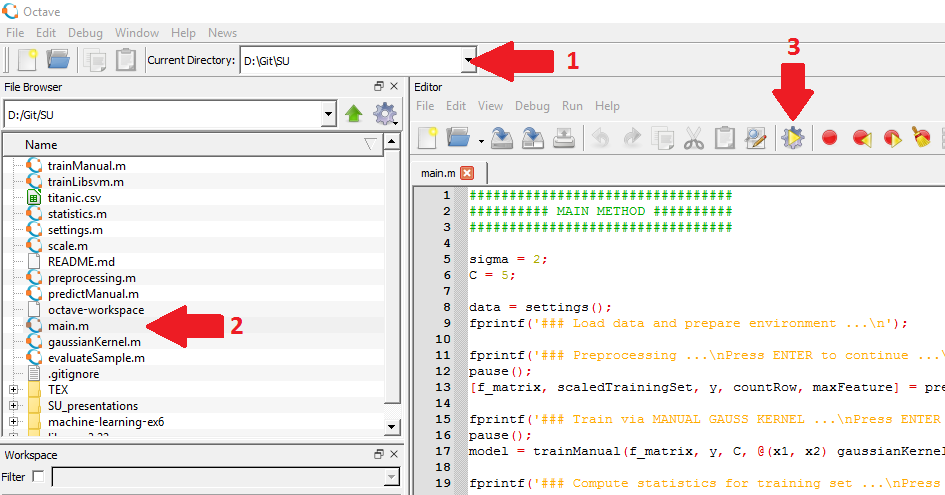
\includegraphics[width=\textwidth]{images/runWithGUI}
	\caption{1. Nastavení cesty do složky programu, 2. Hlavní program (rozkliknout do záložky), 3. Spuštění programu}
	\label{fig:runWithGUI}
\end{figure}

\subsection{Spuštění}
Máme dvě možnosti spuštění:

\begin{enumerate}
	\item - Octave (GUI) : Máme-li Octave ve verzi s GUI, tak po spuštění programu navedeme Octave do správné složky s programem a spustíme modul \texttt{main.m} (viz Obr.:\ref{fig:runWithGUI})
	\item - Octave (CLI) : Spouštíme-li Octave v příkazové řádce, je nutné se přesunout do složky programu s moduly a zadat pouze příkaz \texttt{main} (viz Obr.:\ref{fig:runWithoutGUI}.
\end{enumerate}

\begin{figure}[!ht]
	\centering
		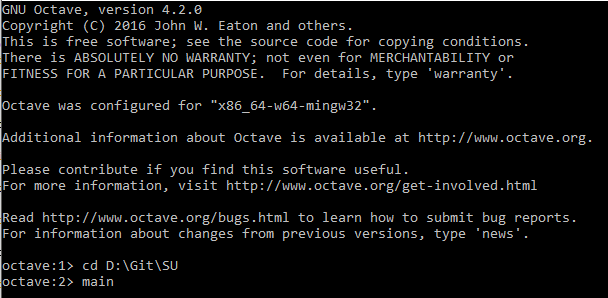
\includegraphics[width=\textwidth]{images/runWithoutGUI}
	\caption{Spuštění Octave (CLI)}
	\label{fig:runWithoutGUI}
\end{figure}

\noindent Dále už průběh pokračuje v obou prostředí stejně. Uživatel je nejprve vyzván, aby postupně zadal vstupní parametry:

\begin{enumerate}
	\item \texttt{Choose SIGMA:} = paramter $\sigma$
	\item \texttt{Choose C:} = parametr $C$
	\item \texttt{Choose size of training set in \%:} = velikost trénovací množiny z původního datasetu. Zbytek data bude použit k validaci správnosti hypotézy.
\end{enumerate}

\noindent Dále stiskem klávesy \texttt{ENTER} spustí načtení a úpravu dat. Jakmile jsou data připravena, spustí se výpočet matice podobnosti indikovaný hláškou \texttt{Similarity ...}. Dokončení výpočtu je značeno hláškou \texttt{... Done!}. Následovně je uživateli vyzván k potvrzení trénování hypotézy. Trénování začíná v okamžiku vyskočení hlášky \texttt{Training ...} a dokončení opět poznáme přes \texttt{... Done!}. Program tedy přejde k výpočtu statistik a zobrazí uživateli v procentech jak moc je hypotéza natrénovaná vůči validačním datům.

\appendix
\begin{thebibliography}{99}

\bibitem{svm_zcu}
EKŠTEIN, Kamil. \textit{Support Vector Machines} [online]. Plzeň, 2012 [cit. 2017-01-31]. Dostupné z: \url{https://portal.zcu.cz/CoursewarePortlets2/DownloadDokumentu?id=123920}. Přednášky k předmětu Strojové učení. Západočeská univerzita v Plzni.

\bibitem{andrew}
NG, Andrew. \textit{CS229 Lecture notes - SVM} [online]. Standford, 2016 [cit. 2017-01-31]. Dostupné z: \url{http://cs229.stanford.edu/notes/cs229-notes3.pdf}. Přednášky k předmětu Machine Learning - CS229. Stanford University.

\bibitem{andrew_new}
NG, Andrew. \textit{Support Vector Machines} [online]. Standford, 2016 [cit. 2017-01-31]. Dostupné z: \url{https://d3c33hcgiwev3.cloudfront.net/_246c2a4e4c249f94c895f607ea1e6407_Lecture12.pdf?Expires=1485993600&Signature=MGhCSj6vnfSMVWpDERGUz8fc2312duxtjEpe2o4R0vhRA9KQQuPnZOPulQy5I0mCrICpxj3M0efelTXkmFFQsKB8VaVCYc0v7qPGH1pnWnL6WdQ1CEkpGAu~i3NfLItowu0Ge3C885eDXuSYBGmDGLUh83obXuukWx9ALN6J5yQ_&Key-Pair-Id=APKAJLTNE6QMUY6HBC5A}. Přednášky k předmětu Machine Learning. Stanford University.

\bibitem{svm_wiki}
Support vector machine. In: \textit{Wikipedia: the free encyclopedia} [online]. San Francisco (CA): Wikimedia Foundation, 2016 [cit. 2017-01-31]. Dostupné z: \url{https://cs.wikipedia.org/wiki/Support_vector_machines}.

\bibitem{svm_robots}
ZISSERMAN, Andrew. In: \textit{SVM dual, kernels and regression} [online]. Oxford, 2015 [cit. 2017-01-31]. Dostupné z: \url{http://www.robots.ox.ac.uk/~az/lectures/ml/lect3.pdf}.

\bibitem{smo_platt}
KEERTHI,S.S.;SHEVADE,S. K.;BHATTACHARYYA,C.;MURTHY,K.R.K.. \textit{Improvements to Platt’s SMO Algorithm for SVM Classifier
Design} [online]. Singapore, 2000 [cit. 2017-02-03]. Dostupné z: \url{http://citeseerx.ist.psu.edu/viewdoc/download?doi=10.1.1.115.5266&rep=rep1&type=pdf}.

\bibitem{smo_platt_original}
PLATT, John C.. \textit{Sequential Minimal Optimization} [online]. Microsoft Research, 1998 [cit. 2017-02-03]. Dostupné z: \url{https://pdfs.semanticscholar.org/8b5e/ab2c9fefe2fb1cc15e755cf7382ffc638f7c.pdf}. A Fast Algorithm for Training Support Vector Machines - Microsoft Research.

\end{thebibliography}
\newpage
\section{Ukázka výstupu programu}
\begin{figure}[!ht]
	\centering
		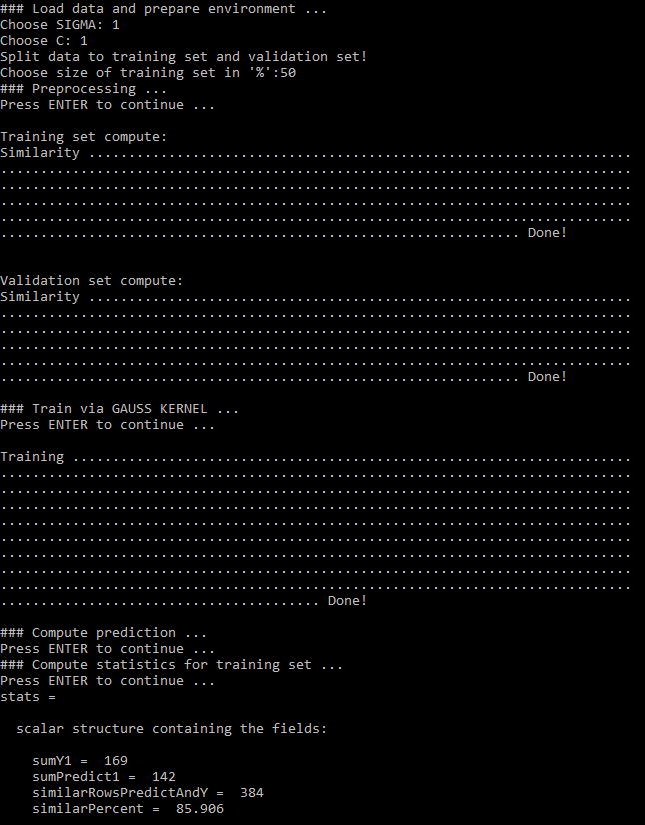
\includegraphics[width=\textwidth]{images/output}
	\caption{Ukázka výstupu programu}
	\label{fig:output}
\end{figure}

\end{document}
